\documentclass[11pt]{article}
\usepackage[margin=1in]{geometry}
\usepackage{amsmath,amssymb,amsthm,graphicx,microtype}
\usepackage[hidelinks]{hyperref}
\usepackage[T1]{fontenc}

\newtheorem{theorem}{Theorem}
\newcommand{\R}{\mathbb R}
\newcommand{\C}{\mathcal C}
\newcommand{\F}{\mathcal F}

\title{A Boundary-Sector Counterexample for Conical Frequency Projection}
\author{Discovery packet for arXiv:0909.3712}
\date{13 August 2026}

\begin{document}
\maketitle

\begin{center}
\fbox{\parbox{0.92\linewidth}{\textbf{Status.}
Full counterexample, pending human review.  The boundary extension asked for
in Remark~5.2 is false: for every $u,v>0$ and every $N>1$ there is
$g\in L^2(\R^2)$ such that $(0,v)$ is $N$-regular for
$P_{\C_{u,v}}g$ but not for $g$.}}
\end{center}

\section{Source question}

Grohs \cite{Grohs} uses the frequency cone
\[
 \C_{u,v}=\{\xi\in\R^2:|\xi_1|\ge u,\ |\xi_2|\le v|\xi_1|\}
\]
and its orthogonal Fourier projection $P_{\C_{u,v}}$. A directed point
$(t_0,s_0)$ is $N$-regular for $f$ when some smooth compactly supported
cutoff $\Phi$, equal to one near $t_0$, and some neighborhood $V$ of $s_0$
satisfy
\[
 |\widehat{\Phi f}(\eta)|=O((1+|\eta|)^{-N})
 \quad\text{whenever }\eta_2/\eta_1\in V.
\]
Lemma~5.1 proves that projection preserves and reflects this property at
interior slopes $s_0<v$. Remark~5.2 asks whether the equivalence remains true
when $s_0=v$.

\begin{figure}[ht]
\centering
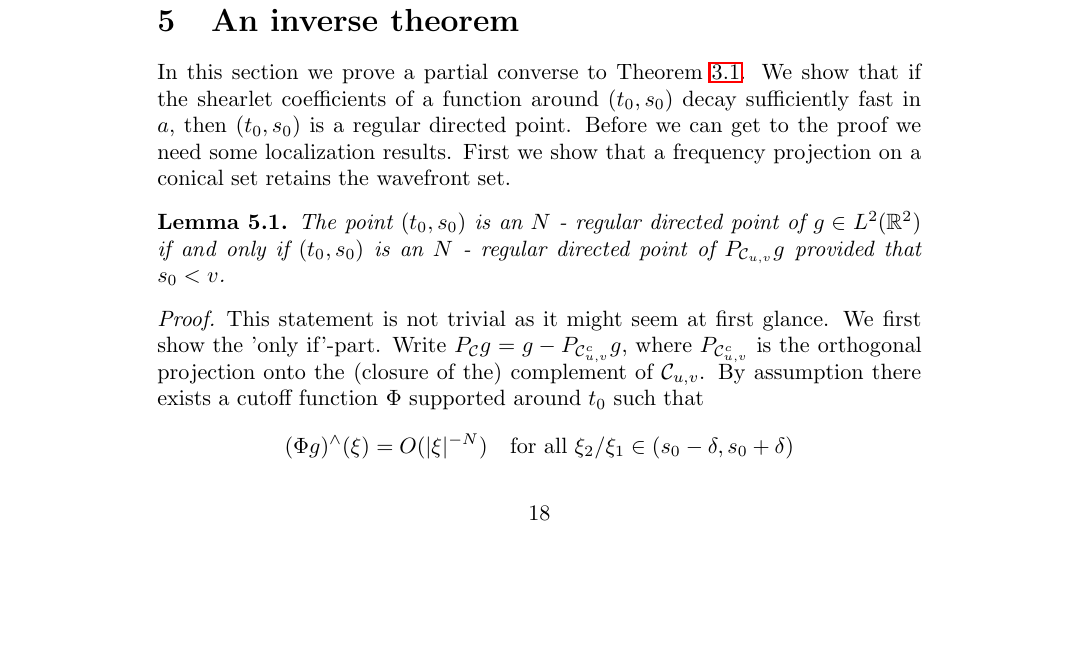
\includegraphics[width=0.485\linewidth]{figures/lemma_5_1_crop.png}\hfill
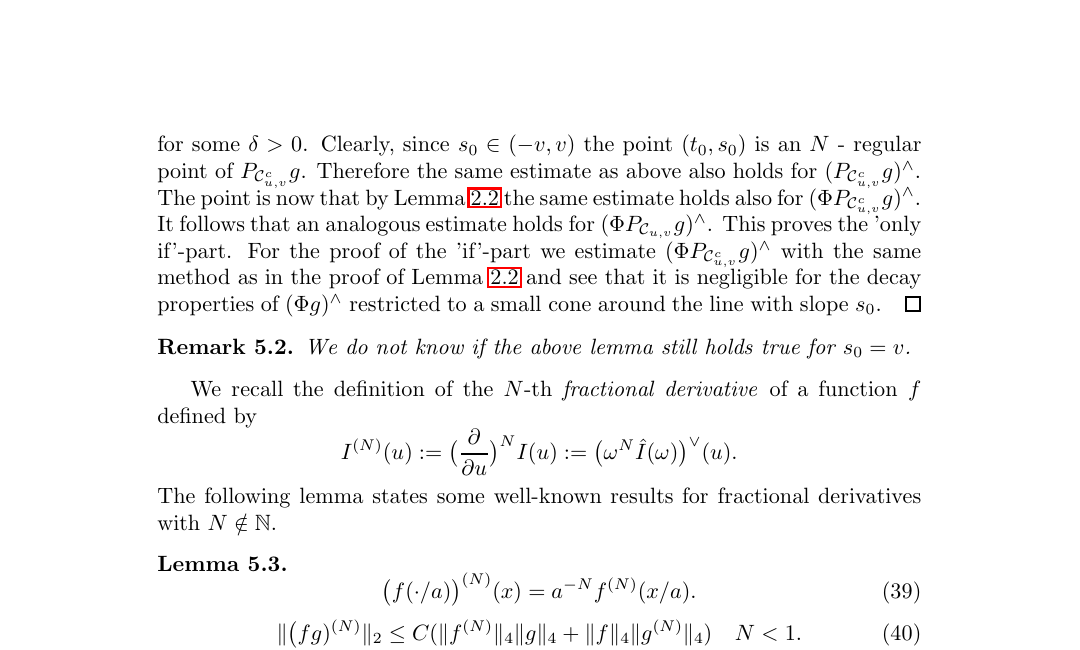
\includegraphics[width=0.485\linewidth]{figures/remark_5_2_crop.png}
\caption{Lemma~5.1 and the boundary question in the source paper
(pp.~18--19).}
\label{fig:source}
\end{figure}

\section{Counterexample}

The obstruction is that every slope neighborhood of $v$ meets the exterior
of the cone. A slowly decaying Fourier sector there is completely deleted by
$P_{\C_{u,v}}$, but its decay survives every spatial localization.

\begin{theorem}\label{thm:main}
Let $u,v>0$ and $N>1$. There exists $g\in L^2(\R^2)$ such that
$P_{\C_{u,v}}g=0$, while $(0,v)$ is not an $N$-regular directed point of
$g$. Consequently the proposed boundary version of Lemma~5.1 is false.
\end{theorem}

\begin{proof}
Choose $\alpha$ with $1<\alpha<N$. Let
$\rho\in C^\infty([0,\infty))$ satisfy $\rho=0$ on $[0,1]$ and
$\rho=1$ on $[2,\infty)$. Choose a nonnegative smooth angular function
$\kappa$ on the unit circle which is supported in
\[
 \{\omega\in S^1:\omega_1>0,\quad
               v<\omega_2/\omega_1<v+1\}
\]
(with support understood in the closure) and is strictly positive at every
direction whose slope lies in the displayed open interval. Such a function
is obtained from the standard flat bump
$\exp(-1/((s-v)(v+1-s)))$ in the slope variable.

Define $h(0)=0$ and, for $\xi\ne0$,
\begin{equation}\label{eq:h}
 h(\xi)=\rho(|\xi|)|\xi|^{-\alpha}
        \kappa\!\left(\frac{\xi}{|\xi|}\right),
 \qquad g=\F^{-1}h.
\end{equation}
In polar coordinates,
\[
 \int_{|\xi|\ge2}|h(\xi)|^2\,d\xi
 \le \|\kappa\|_\infty^2 |S^1|
      \int_2^\infty r^{1-2\alpha}\,dr<\infty,
\]
so $h,g\in L^2(\R^2)$ by Plancherel. The support of $h$ lies outside
$\C_{u,v}$ except possibly on a null boundary, where $\kappa$ vanishes.
Therefore
\[
 \widehat{P_{\C_{u,v}}g}=\mathbf1_{\C_{u,v}}h=0,
 \qquad P_{\C_{u,v}}g=0.
\]
The projected function is thus $N$-regular at every directed point.

It remains to prove that $g$ is not $N$-regular at $(0,v)$. Let $\Phi$ be
\emph{any} smooth compactly supported cutoff equal to one near zero, and let
$V$ be \emph{any} neighborhood of $v$. Choose
$s\in V\cap(v,v+1)$ and set
\[
 e=\frac{(1,s)}{\sqrt{1+s^2}},\qquad c=\kappa(e)>0.
\]
The product--convolution identity gives
\begin{equation}\label{eq:conv}
 \widehat{\Phi g}(Re)=\int_{\R^2}\widehat\Phi(\eta)
                                  h(Re-\eta)\,d\eta.
\end{equation}
We claim that
\begin{equation}\label{eq:asymptotic}
 \lim_{R\to\infty}R^\alpha\widehat{\Phi g}(Re)
   =c\int_{\R^2}\widehat\Phi(\eta)\,d\eta
   =c\Phi(0)=c.
\end{equation}
Indeed, on $|\eta|\le R/2$ one has $|Re-\eta|\ge R/2$; hence
$R^\alpha h(Re-\eta)$ is uniformly bounded and converges pointwise to $c$.
Dominated convergence applies against the Schwartz function
$\widehat\Phi$. On the complementary region, $h$ is bounded and, for every
$K>0$, Schwartz decay gives
\[
 R^\alpha\!\int_{|\eta|>R/2}
 |\widehat\Phi(\eta)h(Re-\eta)|\,d\eta
 \le C_K R^\alpha\!\int_{|\eta|>R/2}(1+|\eta|)^{-K}\,d\eta
 =O(R^{\alpha+2-K})=o(1)
\]
after choosing $K>\alpha+2$. This proves \eqref{eq:asymptotic}.

Thus $|\widehat{\Phi g}(Re)|\sim cR^{-\alpha}$. Since $\alpha<N$, this is
not $O(R^{-N})$. The ray $Re$ has slope $s\in V$, and both $\Phi$ and $V$
were arbitrary. Hence no localization and no slope neighborhood can certify
$N$-regularity of $g$ at $(0,v)$.
\end{proof}

\section{Scope and checks}

The counterexample destroys the ``if'' direction at the boundary:
$P_{\C_{u,v}}g$ is regular but $g$ is not. It does not affect Lemma~5.1 for
strictly interior slopes, where one can choose a slope neighborhood separated
from the exterior sector. The construction is genuinely $L^2$ and uses a
smooth angular cutoff flat at the cone boundary; it does not rely on a delta
mass or another distribution supported on a measure-zero ray.

The quantifiers in directed regularity are essential. Inspecting $h$ alone
would not suffice. Equation~\eqref{eq:asymptotic} proves the obstruction for
every admissible spatial cutoff and every neighborhood of the boundary slope.
The accompanying script checks the support geometry and integrability
exponents; the convolution limit is the analytic heart of the proof.

The paper's other structured-dual question is historically resolved by the
author's follow-up \cite{GrohsTight}, which gives a nonexistence obstruction.
A bounded local-corpus and web search on 13 August 2026 found no explicit
resolution of Remark~5.2 or this sector construction. This is not an
exhaustive novelty claim. Human review should focus on the localization
asymptotic and the novelty status; it has not yet been completed.

\begin{thebibliography}{9}
\bibitem{Grohs}
P. Grohs, \emph{Continuous Shearlet Frames and Resolution of the Wavefront
Set}, arXiv:0909.3712; Monatsh. Math. 164 (2011), 393--426.

\bibitem{GrohsTight}
P. Grohs, \emph{Continuous Shearlet Tight Frames}, arXiv:1001.1516;
J. Fourier Anal. Appl. 17 (2011), 506--518.
\end{thebibliography}

\end{document}
